\section{Analyse post-mortem}
    \subsection{Technologies}
        \subsubsection{Kotlin}
        L'utilisation de Kotlin a été un énorme point positif. En effet, la syntaxe simplifiée de celui-ci a accéléré le développement, amélioré la lisibilité du code et facilité la maintenance du code. Par exemple, les \emph{data classes} de Kotlin permettent d'abstraire en quelques lignes de code des centaines de lignes de Java. De plus, Kotlin est en voie de devenir le langage officiel d'Android; nous étions donc réjouis d'avoir cette occasion d'apprentissage.
        
        \subsubsection{Spring}
        L'utilisation du \emph{framework} Spring n'a pas été appréciée dans le projet, car il y avait trop de magie et de configuration. De plus, ce \emph{framework} était trop lourd. Le temps de démarrage était très élevé malgré que notre projet soit minuscule comparativement à ce qu'un projet avec Spring peut devenir. En rétrospective, l'équipe aurait dû choisir un \emph{framework} Kotlin plus simpliste et plus approprié.

        \subsubsection{Gitlab en déploiement continu}
        Gitlab en déploiement continu fut un élément nettement positif dans notre équipe. Il était si simple de déployer, car tout était automatisé. En effet, il suffisait de fusionner une branche à \emph{master} et Gitlab se chargeait de déployer automatiquement sur les VMs de l'université. En contrepartie, il a été extrêmement complexe d'instaurer cette automatisation. Cependant, nous pensons que l'effort en valait la peine à cause de l'utilisation intensive que nous en avons fait.
        
        \subsubsection{React Native}
        React Native fut un choix controversé dans l'équipe. En effet, celui-ci permet de développer rapidement sur des ordinateurs Windows et Mac pour les plateformes Android et iOS avec un seul \emph{codebase} de manière native. Cependant, React Native est une sorte de dette technique, car éventuellement nous devrons reprogrammer certaines parties de notre application à l'aide des langages natifs si nous voulons atteindre de meilleures performances et plus de personnalisation. En définitive, dans le cadre du projet de session, React Native constituait un avantage net, car notre objectif était de livrer un produit fini avec le plus de fonctionnalités possible en 15~semaines. React Native était le choix parfait pour atteindre les objectifs que nous nous étions fixés.

        \subsubsection{Expo}
        Expo est un outil gratuit et facile d'utilisation qui nous a permis d'accélérer le développement de plusieurs fonctionnalités telles que les notifications. De plus, Expo nous permet de compiler les applications iOS et Android à l'aide d'une seule commande sur Windows ou Mac sans avoir à installer des \emph{toolchains} sur les machines de développement. Expo fut très apprécié par l'équipe et serait à réutiliser si nous refaisions un projet similaire.
        
    \subsection{Gestion}
    Au début du projet nous utilisions Gitlab pour faire la gestion. Cependant, après 30~jours, la version d'essai a expiré et nous nous sommes aperçus bien vite que les fonctionnalités payantes étaient plus que nécessaires pour un bonne gestion de projet. Vu le prix démesuré de Gitlab, nous avons exploré les alternatives et notre choix s'est arrêté sur Jira. Celui-ci coûtait 13~\$ par mois pour toute l'équipe, et nous avons découvert un logiciel qui était bien meilleur que Gitlab. Notre expérience avec Jira a été si positive que nous serions prêt à le réutiliser pour notre projet de fin de baccalauréat ou à le recommander en entreprise.

    \begin{figure}[hp] \centering
        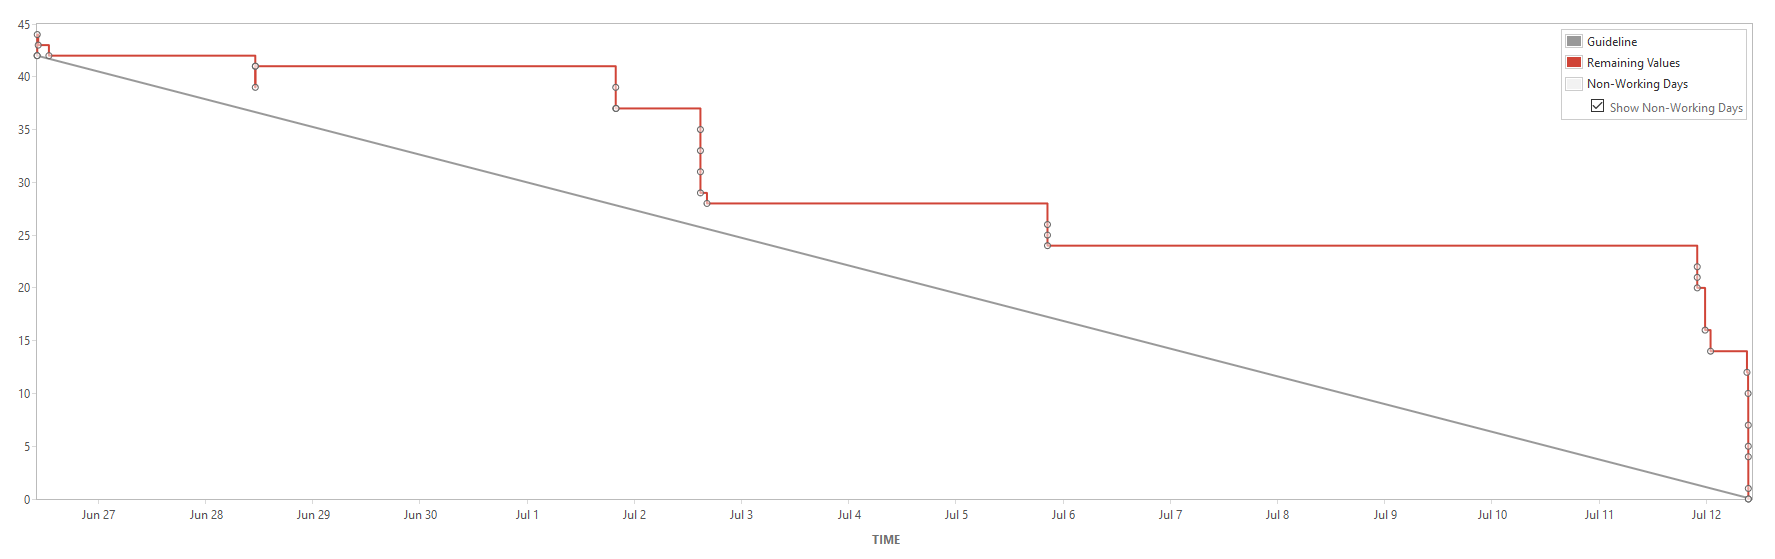
\includegraphics[width=\textwidth]{Figures/burndown}
        \caption{Burndown Chart du troisième sprint du projet}
        \label{fig.burndown}
    \end{figure}

    Le problème principal rencontré par l'équipe consiste en la stagnation du statut des tâches, ce qui avait des répercussions sur le \emph{burndown chart} (figure~\ref{fig.burndown}). Ainsi, lors des réunions, nous avions tendance à fermer beaucoup de tâches d'un coup. On peut aussi remarquer que l'équipe avait parfois de la difficulté à faire avancer le projet en même temps que certains APP plus exigeants. Une division en plus petites tâches et un suivi plus serré sauront régler ces problèmes à l'avenir.

    \subsection{Travail d'équipe et cohésion}
    Le travail d'équipe s'est bien passé tout au long du projet. Étant donnée la grande différences entre les technologies utilisées dans le projet, nous avons commencé à chacun se spécialiser dans un aspect. Par exemple, certain membres de l'équipe s'occupaient des fonctionnalités mobiles en javascript tandis que d'autres faisaient les fonctionnalités du serveur en Kotlin. De plus, même au sein des équipe mobile et backend il y avait des spécialités. Par exemple, au sein de l'équipe mobile, il y avait une personne qui était spécialiste des détails de l'UI.

    Ensuite, l'équipe possédait une très bonne cohésion. En effet, malgré les différents niveaux de compétence, les membres ont travaillé ensemble pour que tout le monde atteigne le même niveau. Il y a donc eu un grand partage de connaissances entre les membres, ce qui s'est avéré essentiel.

    Finalement, nous étions très motivés par notre projet, malgré un relâchement en milieu de parcours. En effet, au milieu du projet nous n'avions pas reçu les accès promis en début de session. Cependant, l'équipe a su contourner cet imprévu en trouvant un moyen alternatif d'avoir un produit fini à temps pour la remise. Cet épisode nous a préparés à la vie réelle, car souvent sur le marché du travail, nous allons faire face à des situation où des fournisseurs ne livrent pas ce qui était attendu et où il faut tout de même livrer un produit fonctionnel.
    